\documentclass[convert,border=2]{standalone}
\usepackage{mathdots}
\usepackage{tikz}
\usetikzlibrary{matrix}
\usetikzlibrary{calc}

\begin{document}
	
	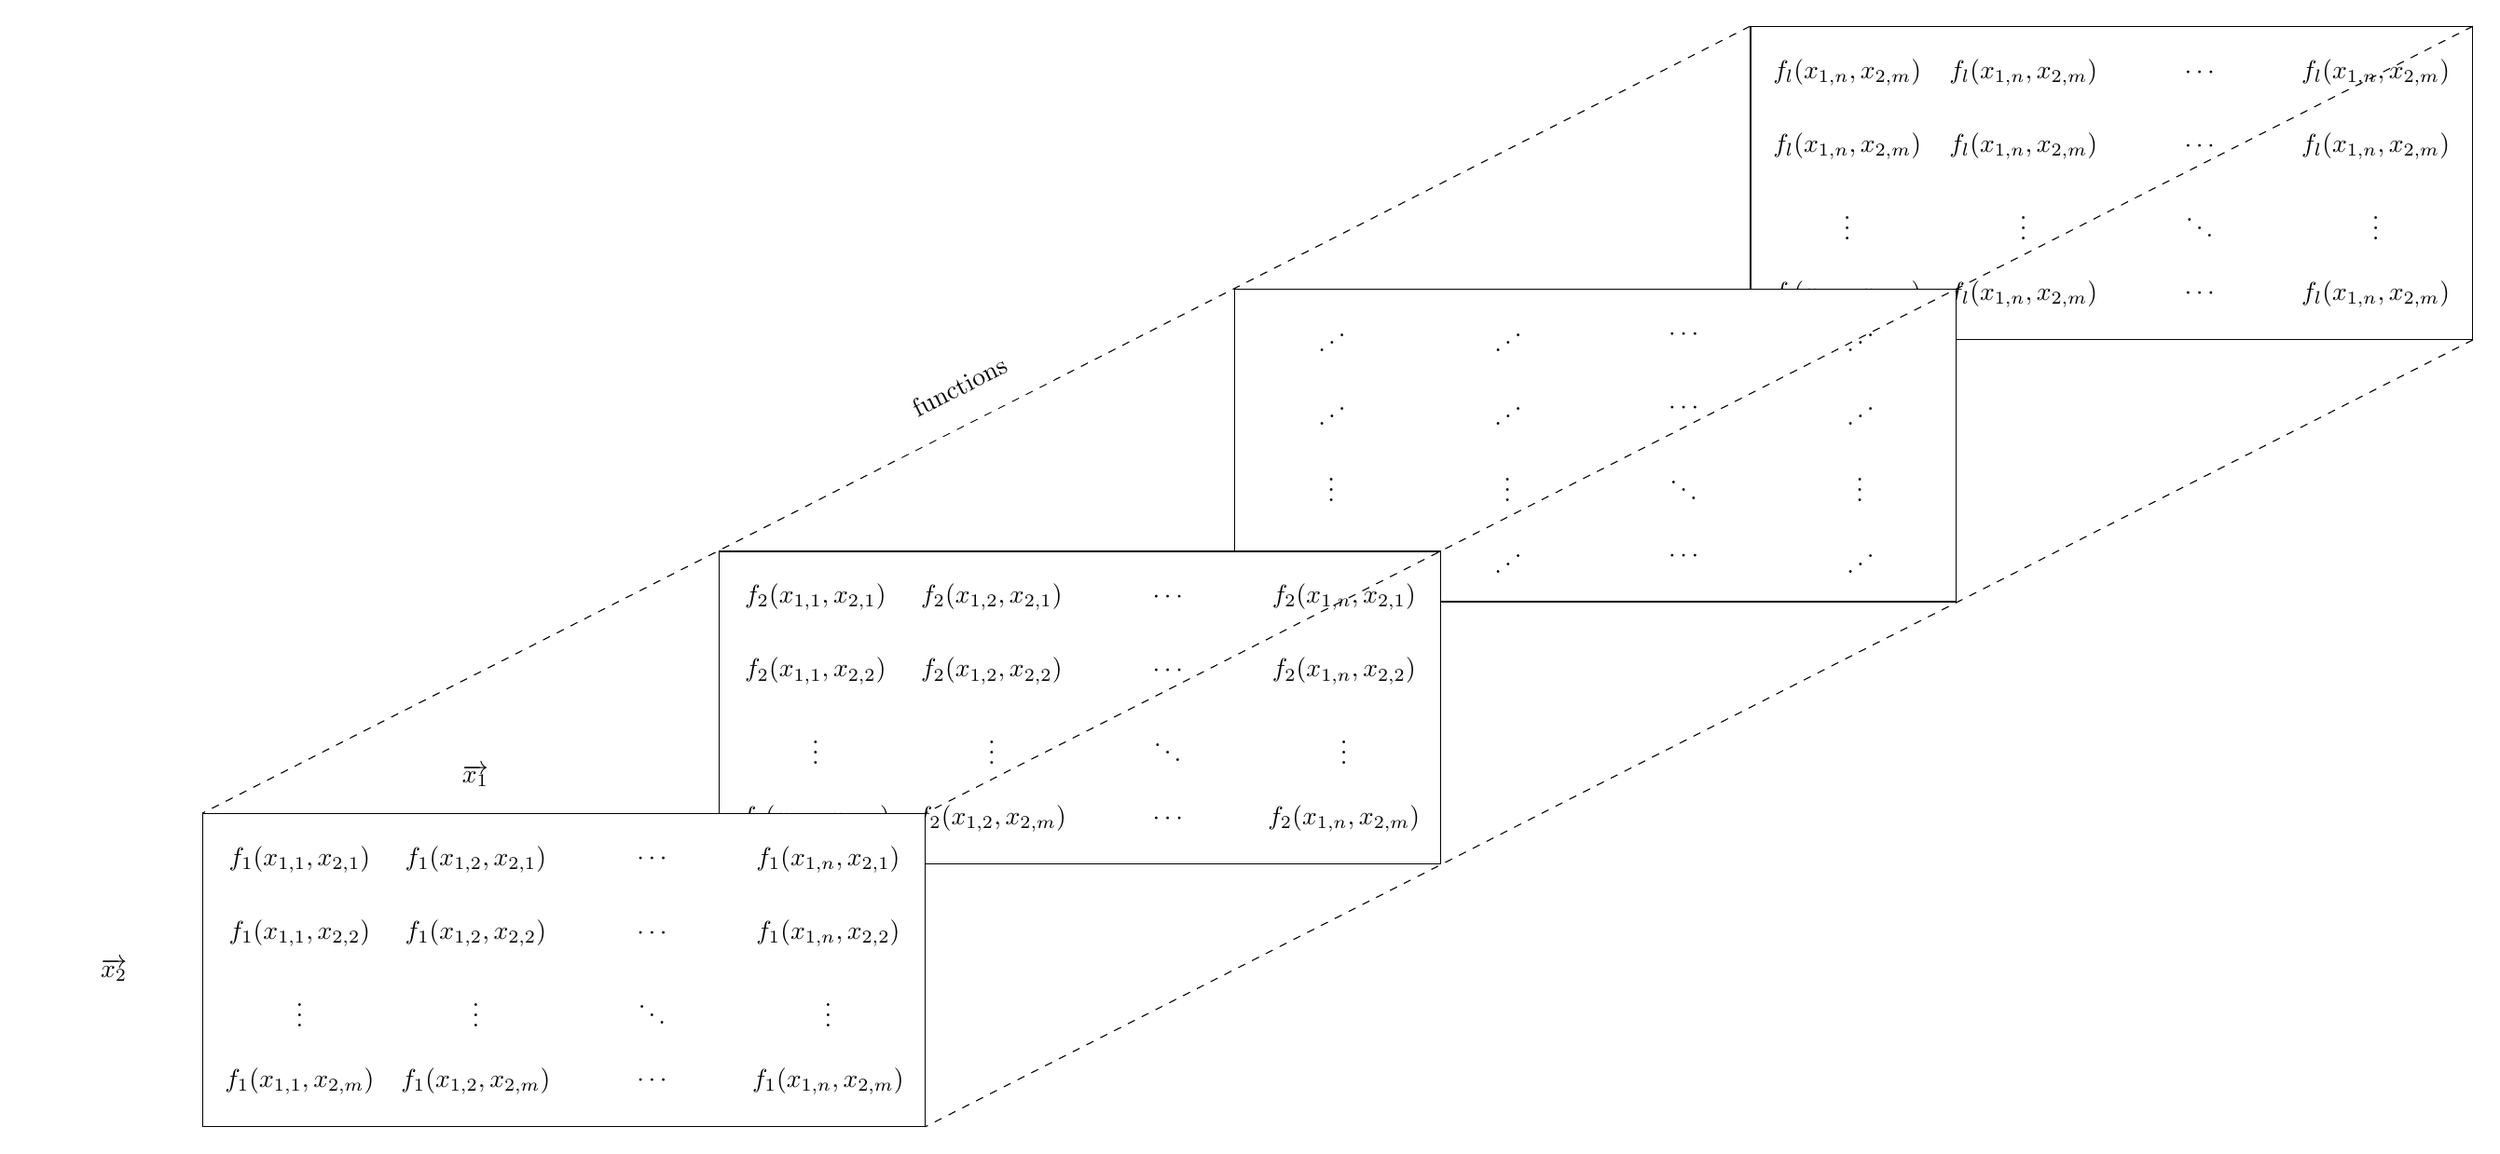
\begin{tikzpicture}[every node/.style={anchor=north east,fill=white,minimum width=2.4cm,minimum height=10mm}]
	\matrix (mA) [draw,matrix of math nodes]
	{ 
		f_l(x_{1,n}, x_{2,m}) & f_l(x_{1,n}, x_{2,m}) & \cdots & f_l(x_{1,n}, x_{2,m}) \\
		f_l(x_{1,n}, x_{2,m}) & f_l(x_{1,n}, x_{2,m}) & \cdots & f_l(x_{1,n}, x_{2,m}) \\
		\vdots  & \vdots  & \ddots & \vdots  \\
		f_l(x_{1,n}, x_{2,m}) & f_l(x_{1,n}, x_{2,m}) & \cdots & f_l(x_{1,n}, x_{2,m}) \\
	};
	
	\matrix (mAd) [draw,matrix of math nodes] at ($(mA.south west)+(2.82,0.7)$)
	{
		\iddots & \iddots & \cdots & \iddots \\
		\iddots & \iddots & \cdots & \iddots \\
		\vdots  & \vdots & \ddots & \vdots  \\
		\iddots & \iddots & \cdots & \iddots \\
	};
	
	\matrix (mB) [draw,matrix of math nodes] at ($(mAd.south west)+(2.82,0.7)$)
	{
		f_2(x_{1,1}, x_{2,1}) & f_2(x_{1,2}, x_{2,1}) & \cdots & f_2(x_{1,n}, x_{2,1}) \\
		f_2(x_{1,1}, x_{2,2}) & f_2(x_{1,2}, x_{2,2}) & \cdots & f_2(x_{1,n}, x_{2,2}) \\
		\vdots  & \vdots  & \ddots & \vdots  \\
		f_2(x_{1,1}, x_{2,m}) & f_2(x_{1,2}, x_{2,m}) & \cdots & f_2(x_{1,n}, x_{2,m}) \\
	};
	
	\matrix (mC) [draw,matrix of math nodes] at ($(mB.south west)+(2.82,0.7)$)
	{
		f_1(x_{1,1}, x_{2,1}) & f_1(x_{1,2}, x_{2,1}) & \cdots & f_1(x_{1,n}, x_{2,1}) \\
		f_1(x_{1,1}, x_{2,2}) & f_1(x_{1,2}, x_{2,2}) & \cdots & f_1(x_{1,n}, x_{2,2}) \\
		\vdots  & \vdots  & \ddots & \vdots  \\
		f_1(x_{1,1}, x_{2,m}) & f_1(x_{1,2}, x_{2,m}) & \cdots & f_1(x_{1,n}, x_{2,m}) \\
	};
	
	\draw[dashed](mA.north east)--(mC.north east);
	\draw[dashed](mA.north west)-- node[sloped,above] {functions} (mC.north west);
	\draw[dashed](mA.south east)--(mC.south east);
	
	\node [above left] at (mC.north) {\overrightarrow{x_1}};
	\node [left] at (mC.west) {\overrightarrow{x_2}};
	
	\end{tikzpicture}
\end{document}